\documentclass[12pt]{article}
\date{May 22, 2019}
\usepackage{pgf-pie}
\usepackage{pgfplots}
\usepackage{pgfplotstable}
\usetikzlibrary{patterns}
\usepackage[section]{placeins}
\usepackage[utf8]{inputenc}

\begin{document}


\clearpage{}
\section{What do you do?}

\label{sec:2}


\begin{figure}[h!]
    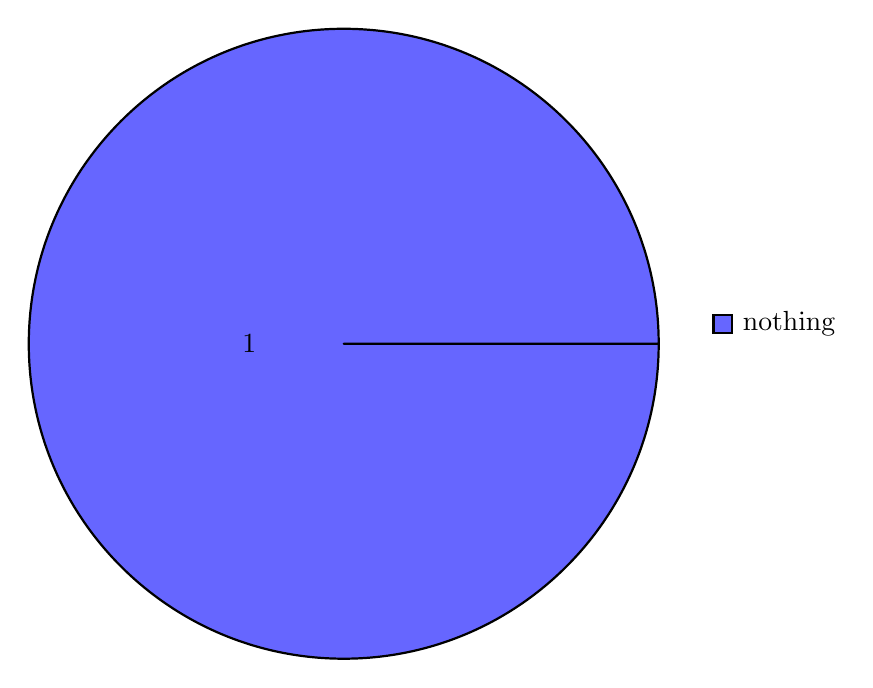
\begin{tikzpicture}
        \pie[radius=4,sum=auto,text=legend]{
            1/nothing
        }
    \end{tikzpicture}
    \caption{\label{figure:q2-1}Repartition of answers for the question 'What do you do?'.}
\end{figure}



\clearpage{}
\section{Testing multiple Choices}

\label{sec:3}


\begin{figure}[h!]
    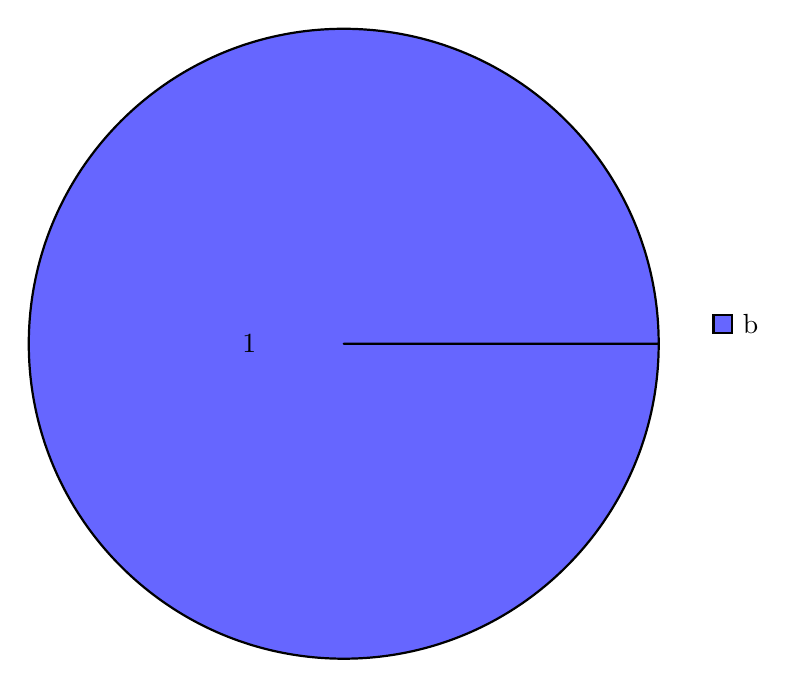
\begin{tikzpicture}
        \pie[radius=4,sum=auto,text=legend]{
            1/b
        }
    \end{tikzpicture}
    \caption{\label{figure:q3-1}Repartition of answers for the question 'Testing multiple Choices'.}
\end{figure}



\end{document}
